\section{The $\Dtwoh$ pitchfork branches}\label{sec:d2h}

Keep $q\in(0,\qc)$, $\mu=p-P_T(q)$ and the gauge $n_u>0$. The $\Dtwoh$ axis of $E_c$ is $a=(s,0,0)$, i.e.\ the
displacement $s\,e_1$.

\subsection{The fixed space}

\begin{lemma}[exact symmetry audit of the $\Dtwoh$ axis]\label{lem:fix}
Let $\Sigma=\{R\in\Oh:D(R)e_1=e_1\}$.
\begin{enumerate}[label=(\alph*)]
\item $\Sigma$ has order $8$ (elements $E$, $C_4^2$, $i$, $\sigma_h$, $2C_2'$, $2\sigma_d$): it is the $\Dtwoh$ with
$C_2$ axes $x$, $(0,1,1)$, $(0,1,-1)$, for every $n$.
\item $\Fix_{\R^{24}}(\Sigma)=\Span\{\Ahat,\Ehat,e_1,f_1\}$ (orthonormal), where $\Ahat=E_{\mathrm{br}}/\sqrt{24}$
($\Aonegg$), $\Ehat(s)=(2s_1,-s_2,-s_3)/\sqrt{48}$ (the tetragonal $\Eg$ strain along the axis), and $e_1,f_1$ are one
direction from each $\Ttwog$ copy. Isotypically,
\[
\Fix(\Sigma)=\Aonegg\oplus\Eg\oplus\Ttwog^{(1)}\oplus\Ttwog^{(2)}\quad(\text{one fixed direction each}),
\]
and no rigid motion is fixed.
\item $b:=D^3V[e_1,e_1,\cdot\,]\in\Aonegg\oplus\Eg$: $b=b_A\Ahat+b_E\Ehat$ exactly, with $\langle b,e_1\rangle=\langle b,f_1\rangle=0$.
\item The $8$ elements of $\Oh$ that map $e_1$ to $-e_1$ form, with $\Sigma$, the normaliser $N(\Sigma)\cong\Dfourh$; each
acts on $(\Ahat,\Ehat,e_1,f_1)$ as $\operatorname{diag}(1,1,-1,-1)$.
\item In the basis $(\Ahat,\Ehat,\uh_1,\vh_1)$ the Hessian restricted to $\Fix(\Sigma)$ is $\operatorname{diag}(h_A,h_E)\oplus K$,
where $h_A$, $h_E$ are the $\Aonegg$ and $\Eg$ eigenvalues of the cube.
\end{enumerate}
\end{lemma}
\begin{proof}
All items are computed exactly from the $\Oh$ action on $\R^{24}$, with $n_u,n_v$ symbolic and a generic pair
potential: the stabiliser from the $48$ matrices, the fixed space from the projector $\frac18\sum_{g\in\Sigma}D(g)$ (rank
$4$) and the ranks of its products with the isotypic projectors, and $b$ as a $24$-vector of linear forms in
$\psi^{(k)}(\sigma)$. For (c) there is also a structural reason: $b$ is the image of $e_1\otimes e_1$ under an
$\Oh$-equivariant map, $\operatorname{Sym}^2(\Ttwog)=(\Aonegg\oplus\Eg)\oplus\Ttwog$, and the $\Ttwog$ component of
$\operatorname{Sym}^2$ is $(a_2a_3,a_3a_1,a_1a_2)$, which vanishes at $(1,0,0)$ (on the $\Dthreed$ axis it does not; this
is the $I_3$ structure seen from the other side).
\end{proof}

\begin{remark}\label{rem:fixspace}
The fixed space contains the noncritical same-axis $\Ttwog$ direction $f_1$ and exactly one $\Eg$ direction (the
strain $\operatorname{diag}(0,1,-1)$ is not $\Sigma$-fixed). An informal description used in early planning,
$\Span\{e_{\mathrm{crit}},\Aonegg,\Eg^{(1)},\Eg^{(2)}\}$, omitted $f_1$ and included a second $\Eg$ direction; only the
dimension agrees. The comparison is recorded in the development documentation of the release package.
\end{remark}

\subsection{The quartic coefficient and Lemma Q}

By \cref{lem:fix}(d) the reduced potential on the axis is even, and $D^3V[e_1,e_1,e_1]=0$. Eliminating
$w\in\Span\{\Ahat,\Ehat,f_1\}$ at second order, with $b\in\Span\{\Ahat,\Ehat\}$ and $\Ahat,\Ehat$ eigenvectors of the full
Hessian, gives
\begin{equation}\label{eq:c4D2h}
c_4=D^4V[e_1^4]-3\langle b,H_\perp^{-1}b\rangle=D^4V[e_1^4]-3\frac{b_A^2}{h_A}-3\frac{b_E^2}{h_E}.
\end{equation}
The denominators are positive for all $p>q>0$ (Paper~2, Lemma~S). The value of \eqref{eq:c4D2h} was confirmed by three
independent routes: the symmetry-adapted formula, a raw $24$-dimensional computation with no symmetry (exact in
SymPy \citep{SymPy2017} for symbolic $n$, and numerically with a spectral pseudo-inverse), and a derivative-free
nonlinear reduction in the four $\Sigma$-orbit coordinates; at five curve points they agree to relative $10^{-36}$ or
better. All terms are difference forms (\cref{app:closed}), each carries the factor $qW_q(p-q)$, and
\begin{equation}\label{eq:c4fact}
c_4=qW_q\,(p-q)\,\cfhat,\qquad
\cfhat=\frac{\widehat Q(1,\rho)-\frac32\,\widehat b_A(1,\rho)^2-3\,\widehat b_E(1,\rho)^2/\widehat h_E}{(1+\rho^2)^2},
\end{equation}
with the divided differences $\hat f$ of \cref{sec:d3d}, the chart $\rho=-\Mhat_{12}/\Mhat_{22}$, $\widehat h_A=2$ exactly, and
$\widehat Q(n)=\sum_j\binom4j n_u^{4-j}n_v^j\widehat Q_j$. Unlike $\kappa$, $c_4$ does not depend on the gauge.

\begin{named}{Lemma Q}[certified]\phantomsection\label{lem:Q}
On the whole closed physical $\Ttwog$ curve ($p=P_T(q)$, $0\le q<\qc$, and the corner $p=q=\qc$), $\cfhat>0$, together with
$\widehat h_E>0$ and $\Mhat_{22}>0$. More precisely $\cfhat\ge955723/262144=3.6457\ldots$ on every curve box,
$\cfhat(0)=3.7993380378\ldots$ and $\cfhat(\qc)=4.3770354906\ldots$. At $q=0$ the divided differences are
$(f(P_T(0))-f(0))/P_T(0)$; at the corner they are the derivatives $f'(\qc)$.
\end{named}

The certificate uses the $222$ curve boxes and $\delta$-balls of the \lemK\ certificate unchanged (hash-pinned), re-verifies
each ball by a strict interval Newton inclusion, encloses the divided differences without dividing by $\delta$, and
certifies both endpoints directly; an independent checker re-derives all functions and uses no Taylor series
(\cref{sec:cert}).

\begin{corollary}[sign of $c_4$]\label{cor:c4}
$c_4(q)=qW_q\,(P_T(q)-q)\,\cfhat(q)>0$ for every $0<q<\qc$, since $q>0$, $W_q>1$ and $P_T(q)>q$ (Lemma~T3). The raw $c_4$
vanishes at both ends through the factors $q$ and $p-q$; no sign of the raw $c_4$ is claimed there.
\end{corollary}

\subsection{Proposition B2}

\begin{named}{Proposition B2}[the $\Dtwoh$ pitchfork]\phantomsection\label{prop:B2}
Fix $q\in(0,\qc)$. Then $\tau<0$ and $c_4>0$. There are $\varepsilon>0$ and $\mu_0>0$ such that for $|\mu|<\mu_0$ the
equilibria of $V_p$ in $\ystar+\Fix(\Sigma)$ within distance $\varepsilon$ of $\ystar$ are exactly
\begin{itemize}
\item the cube, for every $\mu$;
\item for $\mu>0$ only, two further equilibria $x_\pm(\mu)=\ystar\pm s_*(\mu)e_1+w(\pm s_*(\mu),\mu)$ with $s_*(\mu)>0$ and
\begin{equation}\label{eq:ampD2h}
s_*(\mu)^2=-\frac{6\tau}{c_4}\,\mu+O(\mu^2);
\end{equation}
\item for $\mu\le0$, no other equilibrium.
\end{itemize}
$x_+$ and $x_-$ are exchanged by each element of $N(\Sigma)\setminus\Sigma$, and each has isotropy exactly $\Sigma\cong\Dtwoh$ in
$\Oh$. The branch is a $\Z_2$-symmetric pitchfork, supercritical in the reduced-energy axial convention, opening towards
$p>P_T(q)$. Along the axial reduced coordinate, $\partial_s^2\Vred=\tau\mu+O(\mu^2)<0$ at the cube for $\mu>0$ and
$\partial_s^2\Vred=-2\tau\mu+O(\mu^2)>0$ at $x_\pm(\mu)$. The same holds on each of the three $\Dtwoh$ axes.
\end{named}

\begin{proof}
\emph{Reduced equation.} Use orthonormal coordinates $(s,w_A,w_E,w_f)$ along $(e_1,\Ahat,\Ehat,f_1)$ on $\ystar+\Fix(\Sigma)$.
By symmetric criticality the $\Sigma$-symmetric equilibria are the critical points of $V$ restricted to this affine space.
By \cref{lem:fix}(e) the $s$-row of the Hessian is $(k_{ss},0,0,k_{sf})$ with $(k_{ss},k_{sf},k_{ff})=(n^{\mathsf T}Kn,n^{\mathsf T}Kf,f^{\mathsf T}Kf)$; at
$\mu=0$, $k_{ss}=k_{sf}=0$ and the other eigenvalues $h_A$, $h_E$, $k_{ff}=\tr K$ are positive (Lemmas~S, T1). The
Lyapunov--Schmidt solution $w(s,\mu)$ is unique and analytic, with $w(0,\mu)=0$, and $\Vred(s,\mu)=V(\ystar+se_1+w(s,\mu))$.
Each $g\in N(\Sigma)\setminus\Sigma$ maps $(s,w_A,w_E,w_f)$ to $(-s,w_A,w_E,-w_f)$ and preserves $V$, so by uniqueness
$\Vred(-s,\mu)=\Vred(s,\mu)$ and
\begin{equation}\label{eq:VredD2h}
\Vred(s,\mu)=V_0(\mu)+\tfrac12\lambda(\mu)s^2+\tfrac{c_4}{24}s^4+O(s^6,\mu s^4,\mu^2s^2),\qquad
\partial_s\Vred=s\,G(s^2,\mu),
\end{equation}
\[
G(z,\mu)=\lambda(\mu)+\tfrac{c_4}{6}\,z+O(z^2,\mu z,\mu^2),
\]
where $\lambda(\mu)=k_{ss}-k_{sf}^2/k_{ff}=\det K(p)/(f^{\mathsf T}K(p)f)$, so $\lambda(0)=0$ and $\lambda'(0)=\tau<0$
(\cref{lem:tau}), and the quartic coefficient at $\mu=0$ is \eqref{eq:c4D2h}, positive by \cref{cor:c4}.

\emph{Branch side.} $G(0,0)=0$, $G_\mu(0,0)=\tau\ne0$, $G_z(0,0)=c_4/6>0$. By the analytic implicit function theorem the
zeros of $G$ near $(0,0)$ form one curve $\mu=\mu_*(z)$ with $\mu_*'(0)=-c_4/(6\tau)>0$; inverting,
$z=-(6\tau/c_4)\mu+O(\mu^2)$. For small $s\ne0$, $x=\ystar+se_1+w(s,\mu)$ is an equilibrium if and only if $\mu=\mu_*(s^2)>0$,
so no nontrivial equilibrium exists for $\mu\le0$, and for small $\mu>0$ there is exactly one $z>0$ and exactly two
solutions $s=\pm s_*(\mu)$, $s_*=\sqrt z$. The side $\mu>0$ follows from the signs of $\tau$ and $c_4$; flipping either
sign would flip it.

\emph{Pitchfork and convention.} The cube exists for both signs of $\mu$, the pair $\pm s_*$ only for $\mu>0$, and every
$g\in N(\Sigma)\setminus\Sigma$ maps $x_+$ to $x_-$; $N(\Sigma)/\Sigma\cong\Z_2$ acts on the axis by $s\mapsto-s$. In the
reduced-energy axial convention of \cref{rem:supercritical} (with $\nu=-\lambda(\mu)$) the pitchfork is supercritical
because $c_4>0$: the pair exists where the cube's axial reduced curvature is negative, and consists of minima of
$\Vred(\cdot,\mu)$. The type is the sign of $c_4$ and does not depend on the orientation of $p$.

\emph{Axial curvature.} $\partial_s^2\Vred=G(s^2,\mu)+2s^2G_z(s^2,\mu)$. At the cube this is $\lambda(\mu)=\tau\mu+O(\mu^2)$;
at $s=\pm s_*$, where $G=0$, it is $2z(c_4/6+O(z,\mu))=-2\tau\mu+O(\mu^2)$.

\emph{Isotropy.} For every $R\in\Oh$ the rank of $(D(R)-I)[\uh_1,\vh_1]$ is $0$ if $R\in\Sigma$ and $2$ otherwise, and the $\Ttwog$
projector commutes with $D(R)$, kills $\Ahat,\Ehat$ and fixes $\uh_1,\vh_1$. Every point of $\ystar+\Fix(\Sigma)$ with a nonzero
$(\uh_1,\vh_1)$-component therefore has isotropy exactly $\Sigma$; on the branch that component is
$\pm s_*e_1+O(s_*^3)f_1\ne0$.
\end{proof}

\paragraph{Geometry.} The following is what is rigorously supported near the cube.
\begin{itemize}
\item \emph{Point group.} $x_\pm$ have point group exactly $\Dtwoh$ (not $\Dfourh$, not $\Oh$), and the branch stays
$\Dtwoh$-symmetric for all small $\mu>0$.
\item \emph{Not a cuboid.} $\Sigma$ contains only four of the eight diagonal sign matrices, and
$\Fix(\Sigma)\cap\Fix(\Z_2^3)=\Span\{\Ahat,\Ehat\}$, where $\Fix(\Z_2^3)=\Aonegg\oplus\Eg$ is the cuboid family of Paper~2. Since the
$e_1$-component of $x_\pm$ is nonzero, the branch configurations are not cuboids.
\item \emph{First order.} $\pm s_*e_1$ moves vertex $s$ by $\mp\frac{s_*n_u}{4}(0,s_3,s_2)\mp\frac{s_*n_v\sqrt2}{4}(s_1s_2s_3)(1,0,0)$.
The first term maps each cross-section $x=\text{const}$ by $(y,z)\mapsto(y-\varepsilon z,z-\varepsilon y)$,
$\varepsilon=\pm s_*n_u/2$: the square becomes a rhombus (four equal sides, diagonals scaled by $1-\varepsilon$ along
$(0,1,1)$ and $1+\varepsilon$ along $(0,1,-1)$), i.e.\ the cross-sections are sheared, and $x_+$, $x_-$ are the two rhombi
with the diagonals exchanged. The second term translates the two tetrahedra in opposite directions along $x$ with
weight $n_v$, the opposite-translation component of the critical mode ($n_v\approx0.020$--$0.028$ numerically; that
$n_v\ne0$ on the whole curve is not certified).
\item \emph{Second order.}
\[
x_\pm(\mu)-\ystar=\pm s_*e_1+s_*^2(\omega_A\Ahat+\omega_E\Ehat)+O(s_*^3),\qquad
(\omega_A,\omega_E)=-\tfrac12(b_A/h_A,\,b_E/h_E):
\] the second-order corrections lie in $\Aonegg\oplus\Eg$ (a breathing and a
tetragonal strain along $x$), and the $f_1$-component is $O(s_*^3)$.
\end{itemize}

\begin{figure}[t]
\centering
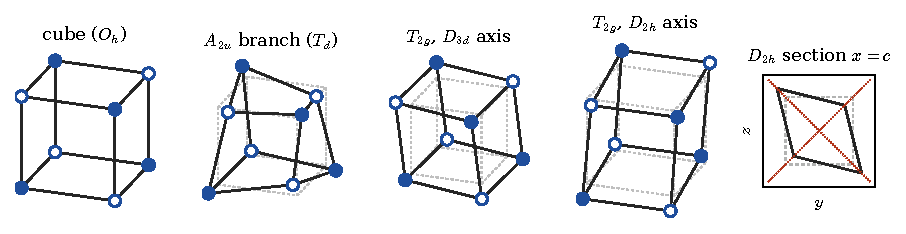
\includegraphics[width=\textwidth]{figures/fig2_modes.pdf}
\caption{First-order shapes of the branch configurations (amplitudes exaggerated; dashed: the cube). Filled and open
circles mark the even and odd tetrahedra. From left: the cube; the $\Atwou$ branch of \thmA, two concentric regular
tetrahedra of unequal radii on inversion-related vertex-direction sets ($\Td$); the $\Dthreed$ branch of \propBone\
(compressed along a body diagonal for $p>P_T(q)$); the $\Dtwoh$ branch of \propBtwo; and a cross-section $x=c$ of the
$\Dtwoh$ branch, in which the square becomes a rhombus (not a rectangle; the configuration is not a cuboid). The
displacements are computed from the exact first-order fields with the kernel vector $n$ at $q=0.8$; the opposite
translation of the tetrahedra (weight $n_v\approx0.025$) is too small to be visible at this scale.}
\label{fig:modes}
\end{figure}

\begin{figure}[t]
\centering
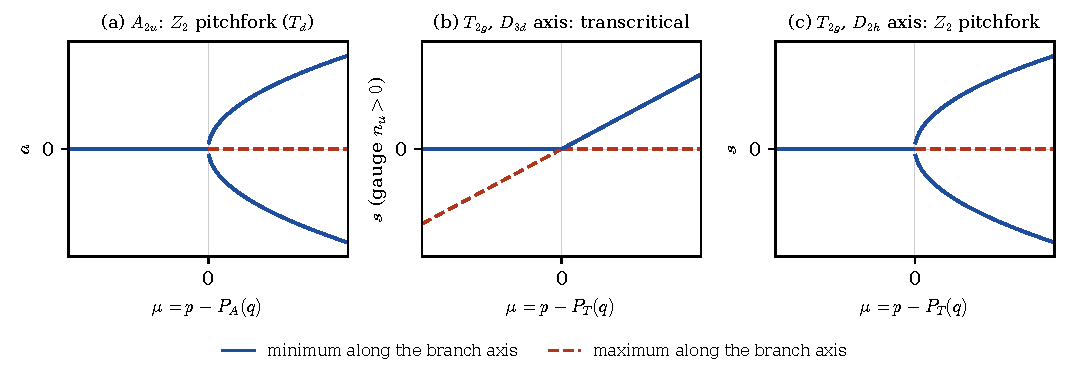
\includegraphics[width=\textwidth]{figures/fig3_bifurcation_diagrams.pdf}
\caption{Local bifurcation diagrams (leading-order normal forms; axes in arbitrary units). (a) $\Atwou$: $a^2\propto\mu$
for $\mu=p-P_A(q)>0$ (\thmA). (b) $\Dthreed$ axis: $s_*=-(\tau/\kappa)\mu$, plotted in the gauge $n_u>0$ where $\kappa>0$,
$\tau<0$ (\propBone). (c) $\Dtwoh$ axis: $s_*^2=-(6\tau/c_4)\mu$ for $\mu=p-P_T(q)>0$ (\propBtwo). Solid and dashed lines mark
minima and maxima of the one-dimensional reduced potential along the branch axis (the reduced-energy axial
convention). This is not stability in $\R^{24}$: the cube is a saddle throughout, and the $\Dtwoh$ branch points have
Morse index $4$ (\corBthree).}
\label{fig:diagrams}
\end{figure}
